\documentclass[10pt]{article}
\usepackage[margin=0.72in]{geometry}
\usepackage{amsmath,amssymb,amsthm,booktabs,graphicx,microtype,placeins}
\usepackage[font=small,skip=3pt]{caption}
\usepackage[hidelinks]{hyperref}
\setlength{\parindent}{0pt}
\setlength{\parskip}{3pt plus 1pt minus 1pt}
\setlength{\textfloatsep}{6pt plus 2pt minus 2pt}
\setlength{\intextsep}{6pt plus 2pt minus 2pt}
\newtheorem{theorem}{Theorem}
\newtheorem{proposition}[theorem]{Proposition}
\newcommand{\AON}{\mathrm{AON}}
\newcommand{\K}{K_{\mathcal L}}
\title{\vspace{-1.8em}\textbf{Semantic Envelopes for Exact}\\[-1pt]
\textbf{Boolean Formula Complexity}}
\author{J. R. Landers}
\date{\vspace{-1.5em}}

\begin{document}
\maketitle
\vspace{-1.7em}

\begin{abstract}
We place exact Boolean formula complexity between two quantities computed from
the truth table: a Khrapchenko boundary obstruction and a decision-tree or
prime-cover construction.  For NAND, NOR, and AND/OR/NOT formulas we prove the
dimension-independent lower bound $B(f)\le K_{\mathcal L}(f)+1$ and elementary
constructive upper bounds linear in minimum decision-tree leaf count $U(f)$.
Exhaustive synthesis of all 65,536 four-input functions yields much sharper
finite envelopes: slopes $9/4$ for NAND/NOR and $13/9$ for AND/OR/NOT.  An
exact weighted prime-cover computation further tightens the latter, giving
$K_{\AON}(f)+1\le\min\{3+\frac{13}{9}(U(f)-1),Q_{\min}(f)\}$.  This cover is
exact for 986 functions, and the combined upper envelope is exact for 1,014.
A compact semantic model predicts exact gate count inside the interval with
held-out $R^2$ of $.946$, $.930$, and $.954$.  The general inequalities and
finite optimal constants are stated separately: the experiment supplies a
sharp small-function benchmark, not a new asymptotic upper bound.
\end{abstract}

\section{From prediction to an interval}

Exact synthesis is practical only for small truth tables, but those tables can
expose structural statements that prediction alone obscures.  Prior exhaustive
work on small Boolean chains and circuits likewise uses exact synthesis to
separate finite optima from general constructions
\cite{haaswijk2017,turan2015}.  Here the target is a tree formula: variables
are free leaves, every gate costs one, fanout is one, and constants are not
free.  We study the bases NAND, NOR, and
$\AON=\{\wedge,\vee,\neg\}$.

For $f:\{0,1\}^n\to\{0,1\}$ let $K_{\mathcal L}(f)$ be its minimum gate
count and $U(f)$ the minimum number of leaves in a deterministic decision
tree.  Write $Z=f^{-1}(0)$, $O=f^{-1}(1)$, and let $E_{01}$ be the
bichromatic edges of the Boolean cube.  Define
\begin{equation}
 B(f)=\frac{|E_{01}|^2}{|Z||O|}
      =\bar s_0(f)\bar s_1(f),
\end{equation}
with $B=0$ for constants.  This is Khrapchenko's classical lower-bound
quantity \cite{khrapchenko1971,jukna2012}.  Our organizing question is not
whether one semantic statistic determines formula size, but where exact cost
lies in the interval between an obstruction and an explicit construction.

\textbf{Contributions.}  We (i) translate the leaf lower bound uniformly to
the three gate-count conventions; (ii) give explicit, if loose, all-$n$
decision-tree upper bounds; (iii) compute sharp affine constants on the full
three- and four-input universes; and (iv) strengthen the AND/OR/NOT endpoint
by exact polarity-weighted prime covers.  Prime-implicant minimization is
classically a set-cover problem \cite{allender2006}; the new role here is as
one endpoint of a basis-specific semantic envelope.

\section{Bounds that hold in every dimension}

\begin{theorem}[Boundary lower bound]
For each $\mathcal L\in\{\mathrm{NAND},\mathrm{NOR},\AON\}$ and every Boolean
function $f$,
\begin{equation}
                  B(f)\le K_{\mathcal L}(f)+1.
\end{equation}
\end{theorem}
\begin{proof}
Replace NAND or NOR gates by their De Morgan forms, and push all negations to
literals.  Do the same for an AON formula.  These transformations preserve
the formula leaves.  Khrapchenko gives $B(f)\le L(f)$ for De Morgan leaf size
$L$.  A rooted formula with $b$ binary gates has $b+1$ leaves; unary NOT gates
only increase total gate count $K$.  Hence $B(f)\le b+1\le K+1$.
\end{proof}

The upper endpoint follows from Shannon expansion.  At a node querying $x$,
\begin{equation}
 f=(\neg x\wedge f_0)\vee(x\wedge f_1),
\end{equation}
which adds four AON gates to formulas for the two children.  A four-gate NAND
multiplexer implements the same recurrence; its De Morgan dual uses four NOR
gates.  Constants cost at most two AON gates and at most five NAND or NOR
gates under our no-free-constants convention.

\begin{proposition}[Constructive tree upper bounds]
For every $f$,
\begin{align}
 K_{\mathrm{NAND}}(f)+1, K_{\mathrm{NOR}}(f)+1
     &\le 6+9(U(f)-1),\\
 K_{\AON}(f)+1&\le 3+6(U(f)-1).
\end{align}
\end{proposition}
\begin{proof}
A binary decision tree with $U$ leaves has $U-1$ internal nodes.  Replacing
each leaf by a constant formula and each internal node by its four-gate
multiplexer gives $K\le5U+4(U-1)$ for NAND/NOR and
$K\le2U+4(U-1)$ for AON.  Adding one yields (4)--(5).
\end{proof}

These constants are intentionally elementary.  They establish a theorem-valid
outer interval against which sharper finite behavior can be measured.

\section{Exact cover endpoint and exhaustive protocol}

For an AON DNF cube $C$, let $\ell(C)$ count literals and $z(C)$ count
negated literals.  The cube costs $\ell-1+z$ gates; joining $m$ cubes costs
$m-1$ OR gates.  Therefore
\begin{equation}
 K_{\mathrm{DNF}}+1=\sum_{C\in\mathcal C}(\ell(C)+z(C)).
\end{equation}
The CNF weight charges the polarity obtained by complementing a zero-cube.
We solve weighted set cover exactly over prime cubes for four forms:
\begin{equation}
 \mathrm{DNF}(f),\quad \mathrm{CNF}(f),\quad
 \neg\mathrm{CNF}(\neg f),\quad \neg\mathrm{DNF}(\neg f),
\end{equation}
and call their minimum $Q_{\min}(f)$.  Retaining one outer NOT is important:
a one-point function can have $K+1=5$ rather than the direct DNF cost $8$.
Positive weights imply that a minimum cover can be chosen from prime cubes.

Exact formula targets are obtained by minimum-layer enumeration.  Initially
the variables have cost zero.  At cost $k$, the algorithm combines only
functions first reached at costs $i$ and $k-1-i$ (and applies unary NOT in
AON).  Every proper subformula of a minimum formula is minimum for its
function, so induction on gate count proves completeness.  The computation
covers all $2^{2^4}=65{,}536$ functions and reproduces an independent
three-input reference table.

For target $Y=K_{\mathcal L}+1$, the largest lower scale and smallest anchored
affine upper slope are computed by
\begin{equation}
 c=\min_{B(f)>0}\frac{Y(f)}{B(f)},\quad
 A=\max_{U(f)=1}Y(f),\quad
 C=\max_{U(f)>1}\frac{Y(f)-A}{U(f)-1}.
\end{equation}
Thus every reported constant is an extremum, not a regression coefficient.
For AON we intersect the exhaustively verified affine curve with the
independently constructive bound $Q_{\min}$.

\section{Sharp small-universe envelopes}

\begin{theorem}[Exhaustive four-input statement]
For every $f:\{0,1\}^4\to\{0,1\}$,
\begin{align}
 B(f)&\le K_{\mathrm{NAND}}(f)+1
       \le6+\tfrac94(U(f)-1),\\
 B(f)&\le K_{\mathrm{NOR}}(f)+1
       \le6+\tfrac94(U(f)-1),\\
 B(f)&\le K_{\AON}(f)+1
       \le\min\{3+\tfrac{13}{9}(U(f)-1),Q_{\min}(f)\}.
\end{align}
The constants $c=1$, $A$, and $C$ are sharp under parameterization (8).
\end{theorem}

\begin{figure}[!t]
\centering
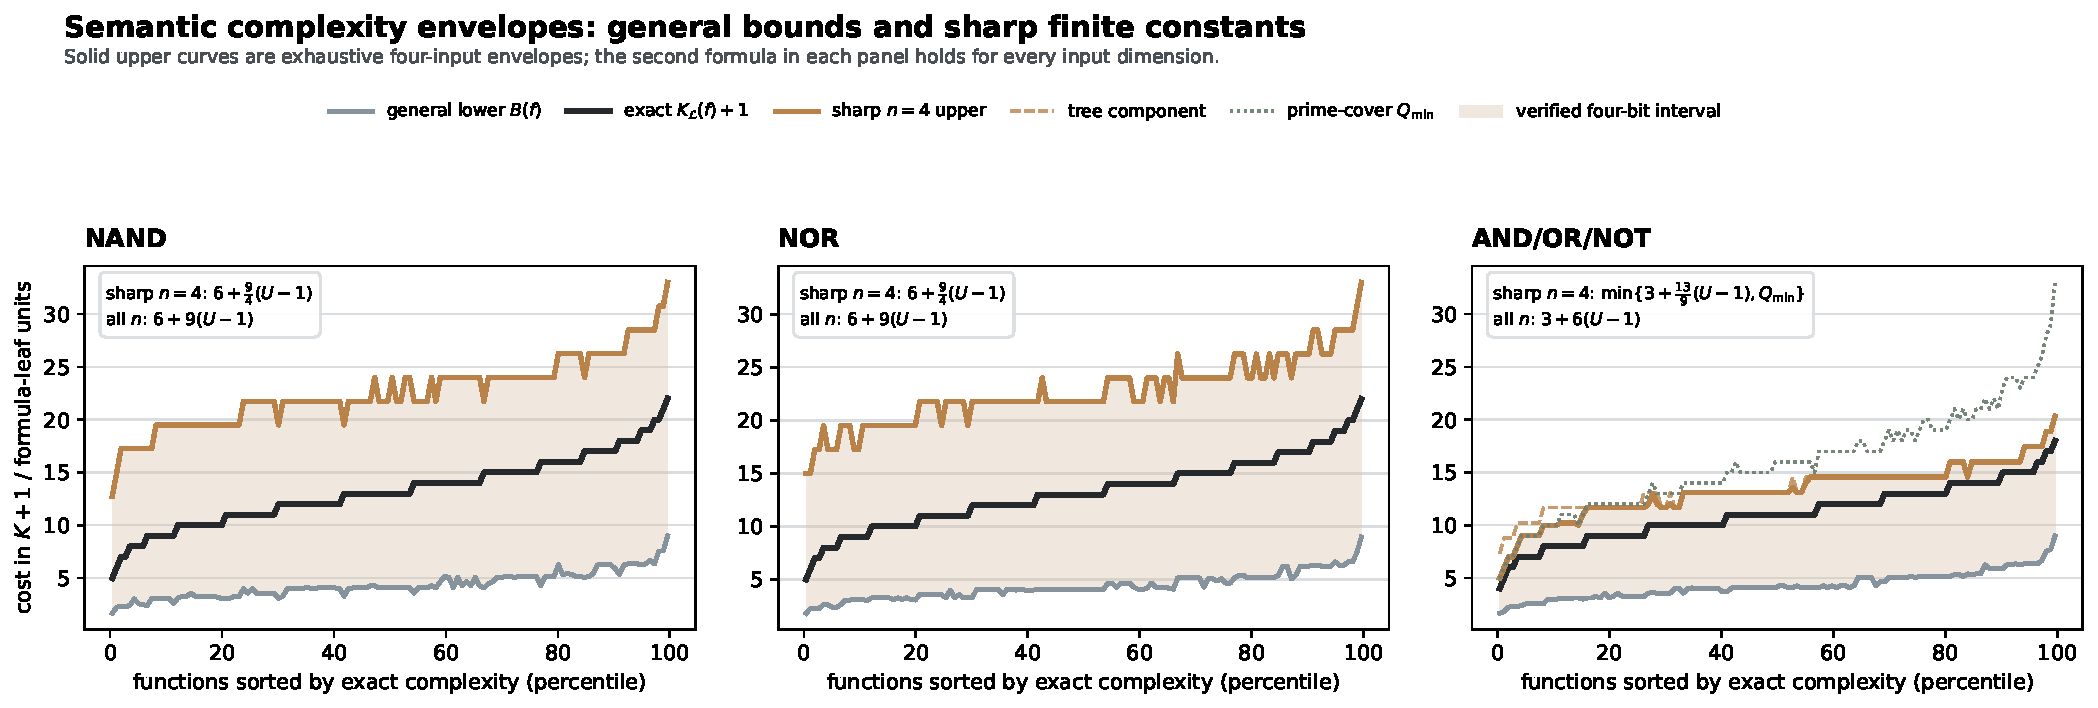
\includegraphics[width=\textwidth]{../../experiments/four_bit/figures/semantic_complexity_envelopes.pdf}
\caption{Median curves in 128 equal-count bins after sorting functions by
exact complexity.  Solid upper curves are the exhaustive four-input
envelopes.  The second formula in each panel is the looser all-$n$ bound.
For AON, the solid endpoint is the minimum of the dashed affine tree curve
and dotted exact prime-cover construction.}
\label{fig:envelopes}
\end{figure}

The lower curve touches exactly the four literals in each four-input basis.
For NAND, the affine upper curve is tight at constant zero and the all-zero
minterm; NOR gives their duals.  In AON, $Q_{\min}$ equals exact complexity
for 986 functions, while the combined endpoint is exact for 1,014.  Four
literal intervals collapse completely: $B=K+1=Q_{\min}=1$.  The 1,026 union
contacts occupy 55 classes under input permutation and output complement;
all representatives and cover witnesses are emitted with the experiment.

\begin{table}[!ht]
\centering\small
\begin{tabular}{clrrrr}
\toprule
$n$ & basis & $c$ & $A$ & $C$ & median width \\
\midrule
3 & NAND/NOR & 1 & 6 & $5/3$ & 9.400 \\
3 & AON      & 1 & 3 & $10/7$ & 3.733 \\
4 & NAND/NOR & 1 & 6 & $9/4$ & 18.600 \\
4 & AON      & 1 & 3 & $13/9$ & 9.156 \\
\bottomrule
\end{tabular}
\caption{Exhaustive constants from (8).  The AON width includes
$Q_{\min}$.  The three-input row is an out-of-sample dimensional check of the
same frozen definitions, not a fit to four-input constants.}
\label{tab:dimensions}
\end{table}

The coefficient-one lower bound and the anchors persist from $n=3$ to $n=4$.
The AON slope changes only from $10/7$ to $13/9$; the NAND/NOR slope increases
from $5/3$ to $9/4$.  This is evidence that the interval is not created solely
by one four-input encoding, but two dimensions cannot establish stabilization.

Finally define normalized position
\begin{equation}
 \rho_{\mathcal L}(f)=
 \frac{K_{\mathcal L}(f)+1-L_{\mathcal L}(f)}
 {H_{\mathcal L}(f)-L_{\mathcal L}(f)}.
\end{equation}
A 16-coordinate model using $(B,U)$, four certificate summaries, five ANF
support counts, and five signed Fourier counts is evaluated by five-fold
holdout of 3,952 complete profile classes.  It reconstructs gate count with
mean held-out $R^2=.946,.930,.954$ for NAND, NOR, and AON, respectively;
position $R^2$ is $.796,.738,.610$.  Tightening the AON endpoint makes
normalized position harder to predict but improves gate reconstruction from
$.950$ to $.954$.

\section{Scope and next theorem target}

Equations (2), (4), and (5) are general proofs.  Equations (9)--(11) are
machine-verified finite statements, and their sharper slopes must not be
extrapolated as asymptotic constants.  Exact-cover equality is also not exact
formula equality in general: factoring can beat every two-level cover.

The result nevertheless replaces an unconstrained prediction problem by a
specific residual question: which semantic properties locate a function
inside a rigorous lower--upper interval?  Certificates describe how quickly
the tree construction terminates; ANF support and Fourier signs distinguish
functions with similar boundary and tree coordinates.  The next decisive
test is to freeze (12) and evaluate selected five-input families---symmetric,
affine, threshold, multiplexer, read-once, and random functions---using exact
targets where feasible and certified intervals otherwise.  A theoretical
advance would either lower the general multiplexer constants toward the
finite slopes or prove that some family forces them away.

\paragraph{What the equality cases say.}
The lower contacts are unusually rigid: in each four-input basis they are
exactly the four positive literals.  The NAND upper slope is forced by the
all-zero minterm together with the constant-zero anchor; NOR is forced by the
dual pair.  The AON endpoint has a different character.  Its 1,014 contacts
include 986 functions for which a prime-cover construction is already an
optimal formula, spread across 55 phase/permutation classes.  The remaining
contacts show where the affine tree coordinate is informative even when no
two-level cover is optimal.  Thus equality is not concentrated in a single
high-symmetry family, and any improved general statement will probably need
to recognize both recursive and cover-like structure.

\paragraph{How the finite claim can fail to scale.}
Three mechanisms could separate higher dimensions from (9)--(11).  First,
decision trees may contain long unbalanced paths, making a uniform affine
coefficient inadequate.  Second, factoring can beat $Q_{\min}$ by an
increasing amount, so the cover endpoint may become systematically loose.
Third, functions with the same $(B,U)$ can differ through algebraic phase or
certificate distribution; the held-out position error already witnesses
this ambiguity at four inputs.  These are concrete failure modes rather than
generic cautions: selected five-input families can test each one separately.
Reporting the first counterexample to a frozen four-input slope would be as
informative as confirming it on a larger class.

\paragraph{Reproducibility.}
All truth tables, exact targets, cover witnesses, equality orbits, folds, and
figure sources are checked in.  The analysis asserts every inequality on all
65,536 functions and includes regression tests for artifact synchronization.

\begingroup
\footnotesize
\setlength{\parskip}{0pt}
\begin{thebibliography}{9}
\setlength{\itemsep}{0pt}
\bibitem{khrapchenko1971}
V.~M. Khrapchenko, ``Method of determining lower bounds for the complexity of
$\Pi$-schemes,'' \emph{Math. Notes}, 10(1):474--479, 1971.
\bibitem{jukna2012}
S. Jukna, \emph{Boolean Function Complexity: Advances and Frontiers}.
Springer, 2012.
\bibitem{allender2006}
E. Allender, L. Hellerstein, P. McCabe, T. Pitassi, and M. Saks,
``Minimizing DNF formulas and $\mathrm{AC}^0$ circuits given a truth table,''
in \emph{Proc. IEEE CCC}, 2006.
\bibitem{haaswijk2017}
W. Haaswijk, E. Testa, M. Soeken, and G. De Micheli,
``Classifying functions with exact synthesis,'' in \emph{Proc. IEEE ISMVL},
2017.
\bibitem{turan2015}
M. S. Turan and R. C. Peralta, ``The multiplicative complexity of Boolean
functions on four and five variables,'' in \emph{LIGHTSEC}, 2015.
\bibitem{buhrman2002}
H. Buhrman and R. de Wolf, ``Complexity measures and decision tree
complexity: a survey,'' \emph{Theor. Comput. Sci.}, 288(1):21--43, 2002.
\end{thebibliography}
\endgroup

\end{document}
